\documentclass[10pt,a4paper,final]{article}

\usepackage[latin1]{inputenc}
\usepackage{amsmath}
\usepackage{amsfonts}
\usepackage{amssymb}
\usepackage{graphicx}

\begin{document}

\section{First Idea}

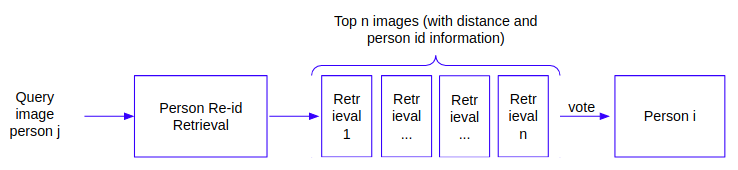
\includegraphics[width=\textwidth]{figures/first_idea.png}

Assuming that the person re-id system goes as specified in figure above, the first idea is to work out the probability $P(class = i \mid query = j)$ by running this on the validation set for each person. It basically states that given a query image of person $j$, how likely that the person is classified correctly as $class = i$. Using this probability we can work out, using Bayesian inference, $P(query=j \mid class=i)$ as:

\begin{equation}
	\label{eq:first_idea}
	\begin{tabular}{r@{=}l}
		$P(query=j \mid class=i)$ & $\frac{\displaystyle P(class = i \mid query = j) P(query=j)}{\displaystyle\sum_{k=1}^{K} P(class = i \mid query = k) P(query=k)}$ \\ 
	\end{tabular}
\end{equation}

\noindent with $K$ the total persons. Given this probability $P(query=j \mid class=i)$, then we can apply partial observability technique to correct the estimate of who the person might be whenever a detection of a person is made.

\section{Second Idea}

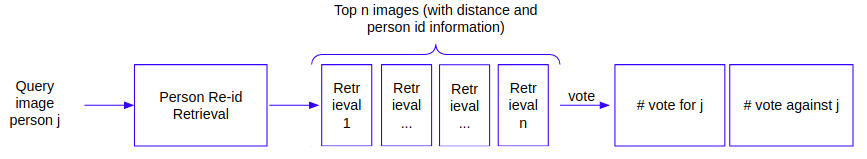
\includegraphics[width=\textwidth]{figures/second_idea.png}

Now, if the person re-id system is specified as in figure above, we can calculate $P(\overrightarrow{v} \mid query = j)$ with $\overrightarrow{v} = (\#vote\_for, ~\#vote\_againts)$ by iterating each image of each person on the validation set. Using this probability we know how likely that the voting goes right (or wrong) given a query of person $j$.

\section{Third Idea}

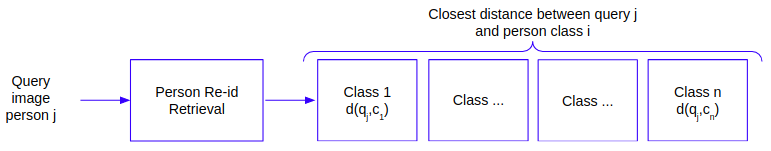
\includegraphics[width=\textwidth]{figures/third_idea.png}

Using the specified re-id system as in figure above with $d(q_j, c_i)$ as the closest distance value between the query of person $j$ and the person classification $c_i$ (the person is classified as $i$), we can calculate the probability $P(distance \mid c_i)$ using the (general) distributions over the distance for both matched image and negative images (graphs given by alex). Using this probability we can work out, using Bayesian inference, $P(c_i \mid distance)$ as:

\begin{equation}
	\label{eq:third_idea}
	\begin{tabular}{r@{=}l}
		$P(c_i \mid distance)$ & $\frac{P(distance \mid c_i) P(c_i)}{\displaystyle\sum_{j=1}^{k} P(distance \mid c_k) P(c_k)}$ \\ 
	\end{tabular}
\end{equation}

\noindent with $k$ the total persons. However, this only works out if the person retrieval system provides the distance $d(q_j, c_i)$ for all $1 \leq i \leq k$ in each query.

\end{document}